\documentclass[a4paper,10pt]{article}
\usepackage[utf8]{inputenc}

\title{Readability}
\author{Sasha and Marco}

\bibliographystyle{plain}



%% PACKAGES %%
\usepackage{latexsym}
\usepackage{amsmath}
\usepackage{amssymb}
%\usepackage{amsthm} %


\usepackage{color}
\usepackage{graphicx}
\usepackage{tikz,pgf}
  \usetikzlibrary{automata,positioning,matrix,calc,petri,arrows}

%% ENVIRONMENTS %%
%\theoremstyle{plain}
%\newtheorem{theorem}{Theorem}
%\newtheorem{lemma}{Lemma}
%\newtheorem{fact}{Fact}
%\newtheorem{example}{Example}
%\newtheorem{definition}{Definition}
%%\newtheorem{corollary}{Corollary}
%\newtheorem{proposition}{Proposition}
%%\newtheorem*{proof*}{Proof}

%% COMMENTS %%

\newcommand\note[1]{{\color{red}{#1}}}
\newcommand{\todo}[1]{{{\color{blue} #1}}}
%\renewcommand{\todo}[1]{}

%% LATEX SHORTCUTS %%
% cause problems with aamas style file
%\def\it{\begin{itemize} }
%\def\-{\item[-] }
%\def\ti{\end{itemize} }
%\def\en{\begin{enumerate} }
%\def\ne{\end{enumerate} }

%% COMPLEXITY CLASSES %%

\def\UPTime{\textsc{up}\xspace}
\def\CoUPTime{\textsc{coup}\xspace}


\def\exptime{\textsc{exptime}\xspace}
\def\exptimeC{\exptime-complete}

\def\pspace{\textsc{pspace}\xspace}
\def\pspaceC{\pspace-complete}

\def\logspace{\textsc{logspace}\xspace}
\def\nlogspace{\textsc{nlogspace}\xspace}

\def\ptime{\textsc{ptime}}
\def\np{\textsc{np}}



%% LOGIC %%
\def\fol{\mathsf{FOL}}
\def\SL{\textsf{SL}}

\def\msol{\mathsf{MSOL}}
\def\fotc{\mathsf{FOL+TC}}

\def\know{\mathbb{K}}
\def\dknow{\mathbb{D}}
\def\cknow{\mathbb{C}}
\def\eknow{\mathbb{E}}

\def\dualknow{\widetilde{\mathbb{K}}}
\def\dualdknow{\widetilde{\mathbb{D}}}
\def\dualcknow{\widetilde{\mathbb{C}}}
\def\dualeknow{\widetilde{\mathbb{E}}}

\renewcommand\implies{\rightarrow}

%% TEMPORAL LOGIC %%
\newcommand{\sqsq}[1]{\ensuremath{[\negthinspace[#1]\negthinspace]}}

\DeclareMathOperator{\ctlE}{{\mathsf{E}}}
\DeclareMathOperator{\ctlA}{\mathsf{A}}


\newcommand{\atlE}[1][A]{\ensuremath{\langle\!\langle{#1}\rangle\!\rangle}}
\newcommand{\atlA}[1][A]{\ensuremath{[[{#1}]]}}

\DeclareMathOperator{\nextX}{\mathsf{X}}
\DeclareMathOperator{\yesterday}{\mathsf{Y}}
\DeclareMathOperator{\until}{\mathbin{\mathsf{U}}}
\DeclareMathOperator{\weakuntil}{\mathbin{\mathsf{W}}}
\DeclareMathOperator{\since}{\mathbin{\mathsf{S}}}
\DeclareMathOperator{\releases}{\mathbin{\mathsf{R}}}
\DeclareMathOperator{\always}{\mathsf{G}}
\DeclareMathOperator{\hitherto}{\mathsf{H}}
\DeclareMathOperator{\eventually}{\ensuremath{\mathsf{F}}\xspace}
\DeclareMathOperator{\previously}{\mathsf{P}}
\newcommand{\true}{\mathsf{true}}
\newcommand{\false}{\mathsf{false}}


\newcommand{\LTL}{\ensuremath{\mathsf{LTL}}\xspace}
\newcommand{\PLTL}{\textsf{PROMPT-}\LTL}

\newcommand{\CTL}{\ensuremath{\mathsf{CTL}}\xspace}
\newcommand{\CTLS}{\ensuremath{\mathsf{CTL}^*}\xspace}
\newcommand{\PCTLS}{\textsf{PROMPT-}\CTLS}
\newcommand{\PCTL}{\textsf{PROMPT-}\CTL}
\newcommand{\CLTL}{\ensuremath{\textsf{C-}\LTL}\xspace}
\newcommand{\PCLTL}{\ensuremath{\textsf{PROMPT-C}\LTL}\xspace}

\newcommand{\ATL}{\ensuremath{\mathsf{ATL}}\xspace}
\newcommand{\ATLS}{\ensuremath{\mathsf{ATL}^*}\xspace}
\newcommand{\PATLS}{\textsf{PROMPT-}\ATLS}
\newcommand{\PATL}{\textsf{PROMPT-}\ATL}

\newcommand{\KATL}{\ensuremath{\mathsf{KATL}}\xspace}
\newcommand{\KATLS}{\ensuremath{\mathsf{KATL}^*}\xspace}
\newcommand{\PKATLS}{\textsf{PROMPT-}\KATLS}
\newcommand{\PKATL}{\textsf{PROMPT-}\KATL}


\def\red{{red}}
\def\col{{col}}
\def\alt{\, | \,}

%% PROMPT 
\def\kmodels{\models^k}
\def\twokmodels{\models^{2k}}
\DeclareMathOperator{\Fp}{\eventually_\mathsf{P}}
\DeclareMathOperator{\Gp}{\always_\mathsf{P}}
\DeclareMathOperator{\within}{\mathsf{within}}

\newcommand{\AP}{{AP}}
\def\Ag{{Ag}}
\def\Act{{Act}}

%% MATH OPERATIONS %%
\newcommand{\tpl}[1]{\langle {#1} \rangle }
\newcommand{\tup}[1]{\overline{#1}}
\def\proj{\mathsf{proj}}
\newcommand{\defeq}{\ensuremath{\triangleq}}

%% STRUCTURES and STRATEGIES %%
\newcommand{\cgs}{\ensuremath{\mathsf{S}}}
\newcommand{\LTS}{\mathsf{S}}
\newcommand{\Comp}{\mathsf{cmp}}
\newcommand{\Hist}{\mathsf{hist}}
\newcommand{\out}{{out}}

\newcommand{\Paths}{\mathsf{pth}}

\newcommand{\nat}{\mathbb{N}}
\def\int{\mathbb{Z}}
\newcommand{\natzero}{\mathbb{N}_0}

\newcommand{\trans}[3]{#1 \stackrel{\mathsf{#3}}{\rightarrow} #2}


%% HEADINGS ETC %%
\newcommand{\head}[1]{\noindent {\bf #1}.}

%% COUNTER MACHINES %%
\newcommand{\cm}{M}
\newcommand{\CMinc}{\mathsf{inc}}
\newcommand{\CMdec}{\mathsf{dec}}
\newcommand{\CMzero}{\mathsf{ifzero}}
\newcommand{\CMnonzero}{\mathsf{nzero}}
\newcommand{\CMcommit}{\mathsf{end}}


%% CLTL %%
\def\var{{\sf var}}
\def\ovar{{\sf ovar}}
\def\avar{{\sf avar}}
\def\svar{{\sf svar}}
\def\bvar{{\sf bvar}}

\def\MOD{\equiv}

%% PVP %%
\def\PVP{\mathsf{PVP}}




\begin{document}

\maketitle

\paragraph{Problem Statement:}
How can one decompose a system that
may be given as a spaghetti mess, into something readable, e.g., a simple
procedural part with declarative modules.

\paragraph{Related question:} Can one mine a readable system from an event log?

\paragraph{Issues:} 
One conceptual difficulty is formalising ``readable''. Let's take as working hypothesis that ``readable'' should be equated with ``succinct as possible'' (in frameworks where the constructs are understandable).

\begin{example}
Suppose we are interested in finite-state systems, i.e., regular languages.
Here are increasingly succinct models: DFA, NFA, AFA, Concurrent AFA. Each is exponentially more succinct than the previous.
Thus, concurrent AFAs are 3exp more succinct than DFAs \cite{DBLP:journals/jacm/DrusinskyH94}. 
\end{example}

\begin{question}
Are automata later in this list more readable then equivalent automata earlier in the list?
\end{question}

Here are some examples which should shed light on this question.

\begin{example}[nondeterminism can improve readability]
Consider the language $L_n$ consisting of all binary strings whose $n$th last bit is $0$. The smallest DFA for this language has about $2^n$ states, while the smallest NFA has about $n$ states. Clearly, to me, the usual NFA for this language is more readable than any equivalent DFA.
\end{example}

\begin{example}[concurrency can improve readability]
Consider the regular language $L_n = \{u\#v : u = v \in \{0,1\}^n\}$.
It has an $O(n^2)$-state concurrent-DFA (the jth component stores the jth bit of u and compares this with the jth bit of v).
But every NFA (and hence every DFA) for $L_n$ requires about $2^n$ states (basically the NFA needs to store the word u in its state).
\end{example}

\begin{example}[concurrency need not improve readability]
Consider the regular language $L_n = \{u : |u| = n\}$. The smallest DFA for this language requires $n$ states and is fairly easy to analyse. 
However, there is a $\log^2 n$ concurrent DFA for this language that is harder to analyse, i.e., it uses $2\log n$ states and the conditions on the edges can be of length $\log n$. This is based on Figure~\ref{fig:counter}.
\end{example}

\begin{figure}
\centering
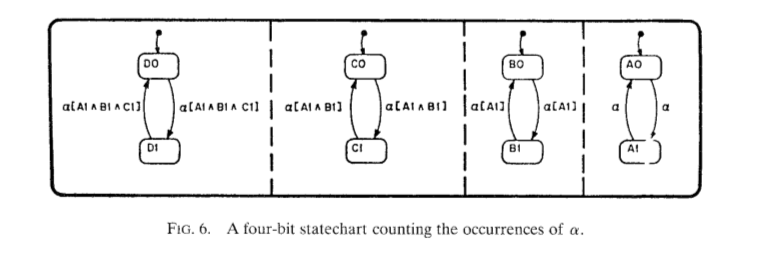
\includegraphics[height=3cm]{counter.png} 
\caption{Taken from \cite{DBLP:journals/jacm/DrusinskyH94}}
\label{fig:counter}
\end{figure}

\begin{example}[concurrent NFAs can be more readable than DFAs]
Consider the regular language $M_n = \{\{0,1,\#\}\#w\#\{0,1,\#\}\$w : w \in \{0,1\}^n\}$. 
The smallest DFA for $M_n$ requires about $2^{2^n}$ states (basically, it needs to remember all substrings of length $n$ that occur before the $\$$, and there are doubly-exponentially many such sets). And thus the smallest NFA for $M_n$ requires about $2^n$ states. However, there is a concurrent AFA of size about $\log^2 n$ for $M_n$. Basically, the AFA nondeterministically guesses the start of $w$; it then branches universally: on the one hand it checks that there the next $\#$ sign is $n$ characters away; on the other, it reads the next bit (until a $\#$ is reached), remembers this bit, and starts a counter that freezes when $\#$ is reached, and resumes when $\$$ is reached, and when the counter reaches $n$ it checks that the bit being read was the one remembered. By the previous example, one can implement a counter up to $n$ with $\log^2 n$ states: 
\end{example}

\begin{question}
 Does mixing alternation and concurrency improve readability?
\end{question}

Finally, a rough/wild idea: using partial observability of $k$ nondeterministic players one can probably save a tower of exponents of height $k$ (this would be based on ideas of \cite{DBLP:conf/focs/PetersonR79}).
% another way to save an exponent is to use partial-observability. Roughly (I need to check the exact details), the idea is that there is an additional equivalence relation $E$ over states; and that if the DFA is in state $q$ then the rest of the word should be accepted from all $q'$ such that $E(q,q')$. This has the advantage that it can be nested; thus with $n$ equivalence relations that form a chain one can save a tower of exponents of height $n$. Finding an example of this that improves readability would be an interesting exercise.

\bibliography{refs}


\end{document}
